\chapter{Implementation}

\textit{This section of the dissertation is focused on the steps involved in constructing, training and evaluating the models 
described in the previous section.
All the models were written from scratch in PyTorch, using the original papers and their implementations as starting points.
This section also covers the tuning of the model hyperparameters, and the subsequent evaluation of the models.}

\section{Model and class structure}

\subsection{PyTorch data structures}
The most important computational unit in PyTorch is the \textbf{tensor}. Tensors are similar to multidimensional arrays, but they are able to 
utilise GPUs to perform operations in parallel. This is important because the running of a neural network involves thousands of matrix 
operations, many of which can be performed in parallel. GPUs have high memory bandwidth and are 
optimised to perform simple operations in parallel, making them ideal for machine learning applications.

Tensors have the property \texttt{requires\_grad} which tells PyTorch whether to record the operations that happen to the tensor. If 
\texttt{requires\_grad=True} the tensor records all operations on it, and builds up a \textbf{computation graph}. The computation graph is a 
directed acyclic graph containing input tensors as the roots and output
tensors as leaves and has \texttt{Functions} as internal nodes. These functions are actually the expressions that are applied to the 
tensors during the forward pass. The graphs are constructed during the forward pass and allow backpropagation to be computed easily by performing a 
backwards pass on the graph to compute the gradients.

\texttt{Parameters} are tensors that hold the weights and biases of the network. The parameter class is a 
wrapper that tells a \textbf{module} whether to include a tensor in the parameters object of the module.

\texttt{Modules} are the base class for all models in PyTorch, and are combinations of parameters and functions that will be applied to input 
data when the \texttt{forward} method of the module is called. All models subclass \texttt{nn.Module} and these modules can be nested
to allow more complicated models to be constructed from basic constituent parts. For example the \texttt{nn.Linear} module contains 
weight and bias parameters, and multiplies the input data by the weights and adds the bias in the forward method.

\subsection{My base modules}
My codebase contains four base modules that are used to construct the more complicated higher-level models. The simplest of 
these base classes are Classifier, Encoder and Decoder.

The Classifier constructor takes as input the dimensionality of the input data, a list of hidden layer sizes, and the number of classes 
in the output, and constructs a simple multilayer perceptron module using \texttt{nn.Linear} for each layer. It uses ReLU as the activation 
function in all the hidden layers and uses a linear function on the output because the implementation of 
cross entropy loss in PyTorch computes log softmax inside it, and so computing softmax in the classifier makes using this incorrect.

The Encoder is very similar to the Classifier, except the constructor also takes in an activation function that is applied to the output 
of the network. This becomes important when the encoder is used in the SDAE. The Decoder constructor is the same as the Encoder to make 
constructing Encoder/Decoder pairs as simple as possible. It takes in the same inputs but reverses them to create the complementary decoder,
also including an output function if required.

The Variational Encoder is a separate module from the Encoder, because the forward pass has three outputs. 
The output of the linear layers is two vectors of the same dimension, $\mu$ and $\sigma$, the parameters of the posterior Gaussian distributions.
It also contains a function that samples from these distributions to create the hidden vector $z$ using the reparameterization trick 
(Appendix~\ref{reparam}). The output of calling \texttt{forward} on the Variational Encoder is then $z$, $\mu$ and $\sigma$.

\subsection{Class structure}

The models used in this project all required certain methods to allow the scripts used for running and evaluation to be as 
model-agnostic as possible. Therefore I implemented a base class \texttt{Model} for all the models to ensure they all had the same methods.
\texttt{Model} also subclassed \texttt{nn.Module} to ensure that the models adhered to PyTorch standards.
\begin{figure}[H]
  \centering
  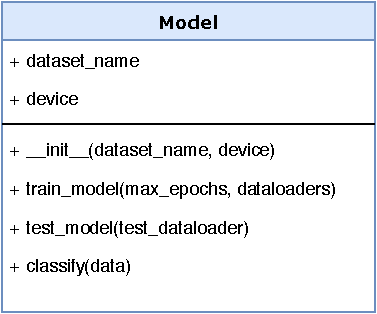
\includegraphics[scale=0.75]{figs/model_class.pdf}
  \caption{Model base class}
\end{figure}

The \texttt{dataset\_name} field is used to save the model state in the correct place when using early stopping, and the \texttt{device} field is 
used to ensure that GPUs are used if available. Not placing the tensors on the correct device 
leads to errors.

Each model has different fields depending on the structure of the model, so initialisation of the models could not be a general method. 
However, for evaluation I implemented a \texttt{hyperparameter\_loop} method per model 
which took the same arguments for all models:
\begin{center}
  \texttt{hyperparameter\_loop(fold, validation\_fold, state\_path, results\_path, dataset\_name, dataloaders, input\_size, num\_classes, max\_epochs, device)}
\end{center}

This method loops through a pre-selected set of hyperparameters to determine the best performing (Section ~\ref{hyper}).

\subsection{Model training}

All the models were trained using mini-batch gradient descent, as described in Section~\ref{batch}.

\subsection{Multilayer perceptron}
The multilayer perceptron is a fully supervised model implemented to compare the performance between a fully supervised approach and the 
semi-supervised approaches used in the project. The model simply uses the Classifier base module and trains it on only the labelled data
using cross entropy loss~\eqref{eq:ce}.

\subsection{M1}
The M1 model described in Section~\ref{m1} is made up of a VAE Encoder,
Decoder and Classifier 
module. The VAE Encoder and Decoder are initially trained in an unsupervised way using both the labelled and unlabelled data. In order 
to train them I chose to normalise all the data to the range [0-1] (Section~\ref{normalise}) and to use a Sigmoid function 
\footnote{the sigmoid function is of
the form $f(x) = \frac{1}{1+e^{-x}}$ and has the domain of the real numbers and range [0-1]} on the output of the Decoder, to ensure the output range 
was the same as the input. This was done for numerical stability reasons, as it was found that using unnormalised or standardised data 
as input to the VAE caused the variance of the latent distribution to become infinitely small and eventually lead to the loss and 
output of the VAE becoming \texttt{nan}.

Once the VAE Encoder and Decoder are trained the Decoder is discarded. The labelled data is passed through the VAE Encoder, and the samples
from the distributions are used as input to the Classifier. The Classifier is then trained on this labelled data using cross entropy 
loss~\eqref{eq:ce}. 

This model relies on the manifold hypothesis. The training of the VAE hopefully clusters similar samples together by finding a lower
dimensional manifold, allowing the Classifier to more easily separate the classes using only a small amount of labelled data.

Once the Classifier is trained the full pipeline for classifying new data involves first passing the data 
through the VAE Encoder and then through the Classifier.

\begin{figure}[H]
  \centering
  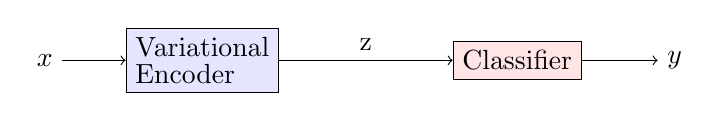
\begin{tikzpicture}
    \node at (0, 0) [black,] (x) {$x$};
    \node at (2, 0) [rectangle,draw,align=left,fill=blue!10] (vae_e) {Variational \\ Encoder};
    \node at (6, 0) [rectangle,draw,fill=red!10] (clas) {Classifier};
    \node at (8, 0) [black, ] (y) {$y$};
    \draw [->] (x) to (vae_e);
    \draw [->] (vae_e) to node[above] {z} (clas);
    \draw [->] (clas) to (y);
  \end{tikzpicture}
  \caption{The classification pipeline of the trained M1 model}
\end{figure}

\subsection{Stacked denoising autoencoder}
The SDAE was constructed by first assembling a list of one-layer Encoders. Each Encoder acts as a linear layer in a classifier,
having the same input size as the latent dimension of the 
previous Encoder. All the Encoders use ReLU as the output activation function, and the final output layer is a simple \texttt{nn.Linear} layer with 
no output activation. This means that passing data through all the Encoders followed by the output layer acts much like 
a Classifier module, but it enables easy unsupervised pretraining.

The unsupervised pretraining is performed by taking each encoder, starting with the first hidden layer, and adding the corresponding 
Decoder. This is where the pairing of the Encoder and Decoder is very useful, as by extracting the layer sizes of the Encoder they 
can be passed straight into the Decoder constructor to create the complementary Decoder. Then Gaussian noise is added to the input data,
using the PyTorch function \texttt{torch.randn\_like(data)}, which creates a Gaussian noise tensor of the same size as the data that can
simply be added to the data. This Encoder/Decoder pair is then trained like a normal autoencoder, training a single layer of the network.

Once each hidden layer has been trained like this, the whole network is trained using labelled data to optimise the network for the 
supervised learning task. Classification involves passing the data through all the Encoders and then through 
the output layer.

\subsection{Semi-supervised VAE (M2)}

The M2 model (Section~\ref{ssVAE}) is made up of a Classifier, a Variational Encoder and a Decoder.
Data is first passed through the Classifier to get a prediction for the label. The loss functions used were given in Section~\ref{ssVAE}, 
and depend on whether the data is labelled or unlabelled. If the data is labelled then the data is passed into the Variational Encoder 
with the correct label, and the output of the Variational Encoder is passed into the Decoder which attempts to reconstruct the data.
If the data is unlabelled then the data and each possible label are passed into the Variational Encoder, and the reconstruction loss 
is computed for all the combinations. If computed iteratively this would greatly increase the training time, but can instead be done 
by creating a larger tensor with every unlabelled sample in the batch paired with each label. This operations on this larger tensor 
can be computed in parallel. The code for performing this 
operation is:

{\renewcommand{\baselinestretch}{0.8}\small
    \begin{verbatim}
      def minus_U(self, x, pred_y):
        # gives probability for each label
        logits = F.softmax(pred_y, dim=1)

        # make a vector of length num_classes*batch_size with each 
        # label repeated batch_size times
        y = self.make_labels(x.size(0))
        # convert label vector to one-hot
        y_onehot = self.onehot(y)
        # repeat data num_classes times (x and y now have same length)
        x = x.repeat(self.num_classes, 1)

        # pass each datapoint with each label through encoder and decoder
        recons, mu, logvar = self.M2(x, y_onehot)
        
        # calculate labelled loss for each pair of datapoint and label (in parallel)
        minus_L = self.minus_L(x, recons, mu, logvar, y)
        # reshape output so all of num_class losses for each datapoint are together
        minus_L = minus_L.view_as(logits.t()).t()
        
        # multiply each labelled loss by the probability of the label
        minus_L = (logits * minus_L).sum(dim=1)

        # compute the entropy of the logits
        H = self.H(logits)

        # calculate -U
        minus_U = H + minus_L

      return minus_U.mean()
    \end{verbatim}
}

The overall structure of the model for unlabelled data is shown below. For labelled data the label passed into the Variational Encoder 
and Decoder comes from the dataset, not the classifier.

\begin{figure}[H]
  \centering
  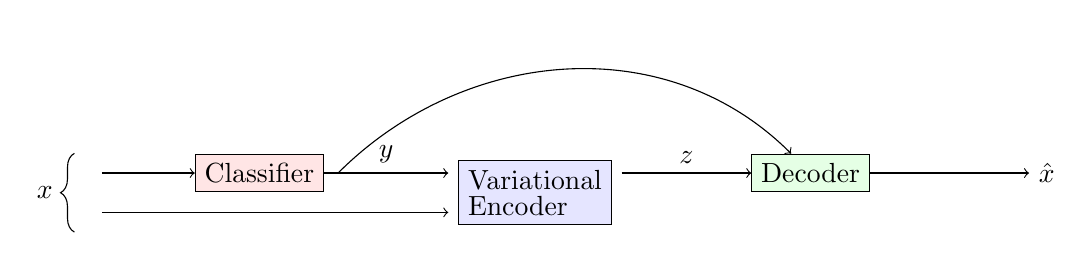
\begin{tikzpicture}
    \node at (2, 0.25) [rectangle,draw,fill=red!10] (clas) {Classifier};
    \node at (5.5, 0) [rectangle,draw,align=left,fill=blue!10] (vae_e) {Variational \\ Encoder};
    \node at (9, 0.25) [rectangle,draw,fill=green!10] (dec) {Decoder};
    \node at (12, 0.25) [black,] (x_hat) {$\hat{x}$};
    \draw [->] (0, 0.25) to (clas);
    \draw [->] (clas) to node[above] {$y$} (4.4, 0.25);
    \draw [->] (0, -0.25) to (4.4, -0.25);
    \draw [->] (6.6, 0.25) to node[above] {$z$} (dec);
    \draw [->] (3, 0.25) to[out=45,in=135] (dec);
    \draw [->] (dec) to (x_hat);
    \draw [decorate,decoration={brace,amplitude=5pt,mirror,raise=-1ex}]
      (-0.5,0.5) -- (-0.5,-0.5) node[left,midway]{$x$};
  \end{tikzpicture}
  \caption{Model structure of M2 for training on unlabelled data}
\end{figure}

The main diffculties in implementing this model came from conflicting information found online. 
The original paper~\cite{DBLP:journals/corr/KingmaRMW14} can be quite hard to decipher, often skipping over difficult derivations, and 
at one point seemingly contradicting itself on the structure of the model.
One of the original blog posts I viewed~\cite{Semisupe95:online} did not pass the label into the 
encoder, and after corresponding with the author I found it was due to a different interpretation of a line in the paper. However,
Kingma's implementation (available at: https://github.com/dpkingma/nips14-ssl) does pass the label into the encoder and so that is the 
model I followed. 

A helpful reference implementation I found is available at https://github.com/wohlert/semi-supervised-pytorch, but I believe my implementation is 
easier to read and also performs better, as I use the inbuilt PyTorch models for computing the cross entropy loss and use the Kingma way 
of computing the KLD~\cite{DBLP:journals/corr/KingmaW13}. I was able to contribute to the repository, finding a bug in the 
variational autoencoder code where the natural logarithm of the variance was restricted to values greater than zero (this is incorrect).

M2 again requires that the data be normalised to the range [0-1] (as in M1) as otherwise the loss explodes and becomes 
\texttt{nan} as the variance of the latent distribution becomes very small.

Once the model is trained the only part used in classification is the Classifier.

\subsection{Ladder} \label{ladder_imp}

The ladder network doesn't make use of any of the base modules, as it requires a lot of extra parts. My original implementation 
was based on an implementation found at https://github.com/abhiskk/ladder. However, this implementation is very slow, as at one point 
tensors on the GPU are unnecessarily shifted onto the CPU to perform operations. The implementation also did 
not achieve the desired accuracy on MNIST. For this reason I instead based my implementation on a Tensorflow implementation written by 
Rinu Boney
(available at https://github.com/rinuboney/ladder), who is a colleague of Rasmus, author of
the 2015 paper~\cite{DBLP:journals/corr/RasmusVHBR15}. The code required extensive rewriting to move from Tensorflow to PyTorch,
but appears to be the fastest and most accurate PyTorch implementation of the model online.

The model is described in some detail in Section~\ref{ladder}, and the overall training process is as below: 
\begin{enumerate}
    \item Data is passed into the clean encoder and the output from each layer is saved.
    \item Data is passed through the noisy encoder, and output from each layer is saved.
    \item The final output from the noisy encoder is the classification output, and supervised loss is computed with it.
    \item The output from the noisy encoder is fed into the decoder. At each layer $l$ of the decoder $g(\tilde{z}^{(l)}, u^{(l+1)})$ is calculated,
          and the unsupervised loss for the layer is computed.
    \item The unsupervised losses are multiplied by hyperparameter $\lambda_{l}$ and summed together.
    \item The supervised and unsupervised losses are summed and backpropagated through the network and the weights are updated.
\end{enumerate}

The Python code used to implement this process is:

{\renewcommand{\baselinestretch}{0.8}\small
    \begin{verbatim}
    for batch_idx, (labelled_data, unlabelled_data) in enumerate(
        zip(cycle(supervised_dataloader), unsupervised_dataloader)):
    self.ladder.train()

    self.optimizer.zero_grad()

    labelled_images, labels = labelled_data
    labelled_images = labelled_images.to(self.device)
    labels = labels.to(self.device)

    unlabelled_images, _ = unlabelled_data
    unlabelled_images = unlabelled_images.to(self.device)

    inputs = torch.cat((labelled_images, unlabelled_images), 0)

    batch_size = labelled_images.size(0)
    
    # pass data through encoders clean
    y, clean = self.ladder.forward_encoders(inputs, 0.0, True, batch_size)
    # pass data through encoders noisy
    y_c, corr = self.ladder.forward_encoders(inputs, self.noise_std, True, batch_size)

    # compute supervised cross entropy loss
    supervised_cost = self.supervised_cost_function.forward(labeled(y_c, batch_size), 
                                                            labels)
    
    # pass output of encoder through decoder
    z_est_bn = self.ladder.forward_decoders(F.softmax(y_c), corr, clean, batch_size)
    zs = clean['unlabeled']['z']
    
    # compute unsupervised reconstruction loss for each layer
    unsupervised_cost = 0
    for l in range(self.L, -1, -1):
        unsupervised_cost += self.unsupervised_cost_function.forward(
            z_est_bn[l], zs[l]) * self.denoising_cost[l]
     
    loss = supervised_cost + unsupervised_cost
    
    # backpropagate loss through network and update weights
    loss.backward()
    self.optimizer.step()
    \end{verbatim}
}

For the most part this was implemented without difficulty, though I did discover early on that the loss sometimes became \texttt{nan}.
By adding a backward hook to the model that notified me when the values became \texttt{nan}, I discovered that this was because 
the ladder requires the data be standardised (Section~\ref{normalise}), which involves dividing the features in the data by the standard deviation of the 
features. However, in the MNIST dataset the pixels on the edge of the images are always black, and so have a constant value of zero over 
all the images. The standard deviation of these features is therefore also zero, and dividing by this leads to data becoming \texttt{nan}.
This can be fixed by adding a small positive value to the denominator when standardising.

\section{Hyperparameter optimisation} \label{hyper}
While the weights and biases in a network can be trained by backpropagation, there are parameters of the model that cannot be trained in 
this way, but still affect the performance of the network. These are hyperparameters and they are set before the training begins. 
Optimising these can be crucial in optimising a model's performance.

\subsection{Grid search}
The most common method for hyperparameter optimisation, and the one used in this project, is grid search. The researcher provides several 
likely values for the hyperparameters, and the model is trained with each combination of these. A validation set is used to compare the
performance of the models, and the best set of hyperparameters is selected in this way.

However, optimising hyperparameters this way results in every combination having to be run again for each additional value of each
hyperparameter used. Depending on how long it takes each model to train, this can significantly prolong training time. 
Therefore, I chose to optimise over a small number of hyperparameters that I felt were most likely to affect the performance of the models.

\subsection{Number of hidden layers}
The number of layers in a model is important because it controls the capacity~\cite{Goodfellow-et-al-2016} of the neural network. If the 
capacity is too high it can \textbf{overfit} to the training data, resulting in poor generalization to new examples, and if the capacity is 
too low it can \textbf{underfit}, resulting in poor fitting to the data. Choosing the number of layers is thus an important hyperparameter.
The universal approximation theorem states that a neural network with a single hidden layer can approximate any function~\cite{DBLP:journals/mcss/Cybenko92}, but the layer 
has to be exponentially large to give the same capacity as a multi-layer network; instead adding new layers is the preferred method, 
with the deeper layers learning more complex and relevant features.

\subsection{Hidden layer size}
Larochelle et al.~\cite{DBLP:journals/jmlr/LarochelleBLL09} found that neural networks with constant layer size usually perform better than
those where the layer size increases or decreases throughout the network. When optimising the number of layers I use a constant layer size
for each hidden layer.

Bengio et al.~\cite{DBLP:series/lncs/Bengio12} found that using a first hidden layer larger than the input layer often resulted in 
better performance. However due to the high dimensionality of gene expression data (over 20,000 genes in the TCGA data) I decided against 
this. 

I use a constant layer size for all the hidden layers, and for all the different models to allow for a fairer
comparison.

\subsection{Latent dimension of autoencoders}
The size of the latent dimension for an autoencoder affects the quality of the representation learned. If the dimension is too small the 
autoencoder may not be able to encode all the important features, whereas a latent dimension that is too large can give the autoencoder 
too much freedom, causing it to not cluster important samples together.

This hyperparameter is only optimisable for the M1 and M2 models, as the hidden dimensions for the autoencoder in the SDAE and ladder 
are controlled by the layer size and number of classes.

\subsection{Learning rate}
The learning rate is a hyperparameter that controls how large a step is taken each time the weights are updated. It is an often
optimised hyperparameter because if it is too large it can overshoot loss minima, resulting in worse performance, and if it is too 
small it can take a very long time for the gradient descent to converge. However, 

I chose not to search over different learning 
rates because of the additional time it would take, and because I used the \textbf{Adam optimizer}. The Adam optimizer keeps a 
learning rate per parameter, and updates these learning rates with respect to each 
parameter~\cite{DBLP:journals/corr/KingmaB14}. This means that while an initial learning rate still has to be provided, it affects the 
performance much less.

\subsection{Early stopping}
The number of epochs that a learning algorithm is trained for also affects how well it performs. Not training for long enough can result in
poor peformance and underfitting, as the model has not had enough time to learn the relevant features. Conversely training for too long can
be waste compute time or even lead to overfitting.

Luckily, this is one of the easiest hyperparameters to optimise, and does not have to be included in a grid search. 
By using a validation set that the network is not trained on, the performance of each model on unseen data can be measured after 
every epoch. Unseen data is necessary because evaluating a model on training data will give overfitted models excellent performance, 
while the actual model generalises poorly and is unusable.
If the performance has improved, the state of the model is saved. After a certain number of epochs without the performance improving, 
the training is stopped, and the best performing model state is loaded.

\subsection{Chosen hyperparameters}

All the models were implemented with early stopping. The simple MLP, SDAE and ladder were optimised over the number of layers in the classifier, using a constant layer size between the input and output size. M1 and M2 were optimised over the number of layers in the VAE, the number of layers in the classifier, and the size of the latent dimension.

\section{Data processing}
An important part of a machine learning project is the pre-processing of the data. This is used to ensure good model performance and 
to partition the data to allow unbiased evaluation.

\subsection{Datasets}
\subsubsection{MNIST handwritten digit database}
The MNIST dataset is one of the most popular in machine learning, being used to benchmark new models in many papers. In this project it is 
also used for benchmarking, and for ensuring that the models are performing similarly to their original implementations.
\begin{table}[H]
  \label{tab:mnist}
  \small % text size of table content
  \centering % center the table
  \begin{tabular}{lccr} % alignment of each column data
  \toprule[\heavyrulewidth]
  Samples & 60,000 train \& 10,000 test \\
  Inputs & 28x28 b/w images  \\
  Number of classes & 10 - digits 0-9 \\
  Balanced & Yes \\
  \bottomrule[\heavyrulewidth] 
  \end{tabular}
  \caption{MNIST dataset} 
\end{table}

\subsubsection{The Cancer Genome Atlas}
The Cancer Genome Atlas is a project cataloguing sequencing data for several different types of cancer. The data generated by the TCGA Research 
Network (https://www.cancer.gov/tcga) is available online at https://portal.gdc.cancer.gov. In this project I used data generated using 
RNA-Seq to attempt to classify the different types of cancer using only their gene expression.
\begin{table}[H]
  \label{tab:tcga_dataset}
  \small % text size of table content
  \centering % center the table
  \begin{tabular}{cc} % alignment of each column data
  \toprule[\heavyrulewidth]
  Samples & 11,060 \\
  Inputs & 20,350 genes with values given as $\log_{2}(\text{TPM}+1)$ \footnotemark \\
  Number of classes & 33 - different cancer types\\
  Balanced & No \\
  \bottomrule[\heavyrulewidth] 
  \end{tabular}
  \caption{TCGA dataset} 
\end{table}
\footnotetext{TPM is transcripts per million, where the total number of reads mapped to a gene is normalised by the length of the gene} 

\subsection{Data normalisation} \label{normalise}
Data normalisation can help neural networks by allowing gradient descent to reach a minimum more easily. Features having large ranges
can result in larger gradients of the loss, resulting in larger steps being taken. This can cause the 
gradient descent to oscillate around minima and take far longer to reach a good value. The two most common forms of data normalisation 
are standardisation and normalisation to the range [0-1]. Having all the features with similar scales is also important for saliency computation
(Section~\ref{saliency}),
as different scales result in different gradients of the output with respect to the input, preventing them from being directly comparable.

\begin{itemize}
  \item \textbf{Standardisation} involves scaling all the features so that they have mean 0 and variance 1. This is done by computing the mean 
          and standard deviation of the features from the training set, and then subtracting the mean from each feature and dividing by the
          standard deviation.
          \begin{align}
            x_{std} = \frac{x - \mu_{x}}{\sigma_{x}}
          \end{align}
  \item \textbf{Normalisation} into the range [0-1] is done by finding the maximum and the minimum for every feature from the training set,
          subtracting the minimum from every feature and dividing by the maximum minus the minimum.
          \begin{align}
            x_{norm} = \frac{x - x_{max}}{x_{max} - x_{min}}
          \end{align}
\end{itemize}

For the MNIST dataset I used normalisation, as the pixels take values between 0 and 255 and so scaling this to be between 0 and 1 is 
simple. It is also the transform used in the code for the ladder network paper~\cite{DBLP:journals/corr/RasmusVHBR15}, 
and similar to the transform used in the semi-supervised VAE paper~\cite{DBLP:journals/corr/KingmaRMW14} (here they set pixel values to 
either zero or one, without the range inbetween).

For the gene expression datasets I tried both standardisation and normalisation. Standardisation worked well for the non-VAE based models,
but the M1 and M2 models experienced significant numeric instability. This is a common problem in
VAEs, especially when the dimensionality of the data is higher than the number of samples in the dataset. The VAEs responded well to normalised
data, while the other models experienced similar or worse performance. Therefore standardisation was used for the MLP, SDAE and ladder 
network and normalisation was used for M1 and M2.

\subsection{Data imputation} \label{imput}
The TCGA dataset contains the gene expression levels for 20,350 genes, but in many of the samples some of these genes are missing.
This can be dealt with by simply discarding the samples with missing genes, but removing such
a large chunk of the dataset is not a good way to improve a model. Instead it may be possible to impute the missing genes, or drop the 
genes, reducing the number of features but keeping the number of samples. In Section~\ref{imputation} there is a comparison 
of the effects of dropping the genes, replacing the missing values with the feature mean, and replacing the missing values with zero.

\subsection{Data partitioning} \label{part}
\subsubsection{Evaluating models and hyperparameter optimisation}
Evaluating the performance of a machine learning algorithm should be done on a test dataset that is separate from the dataset the 
algorithm is trained on, to prevent overfitting leading to overestimating the performance of the model. If the dataset is not particularly 
large this can be done using 
\textbf{$k$-fold cross validation}, where the data is split into $k$ different partitions. $k-1$ of these partitions are used for training, 
while the $kth$ is used to test the performance after training. The accuracy for the model is then computed by taking the average of all
the accuracies for each fold.

\begin{figure}[H]
  \centering
  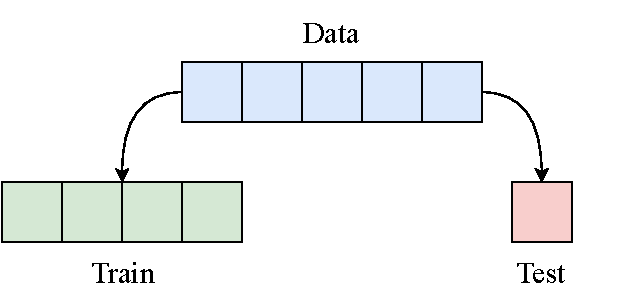
\includegraphics[scale=0.6]{figs/k_fold.pdf}
  \caption{One split of 5-fold cross validation}
\end{figure}

The $k$-fold cross-validation used in this project is \textbf{stratified}. This keeps the proportion of each class in each fold
close to the proportion of each class in the overall dataset. This is especially important when classes are unbalanced, as performing 
non-stratified cross-validation could result in biasing the model towards an uncommon class, or not including any samples of a class in the 
fold. Kohavi~\cite{Kohavi:1995:SCB:1643031.1643047} has shown that stratified cross-validation generally has lower bias and variance when estimating model 
accuracies.

Hyperparameter optimisation (Section~\ref{hyper}) requires a validation dataset, to 
compare the performance of each set of hyperparameters. Performing hyperparameter optimisation on the test set will lead to overestimating 
the ability of the model to perform on unseen data, as the hyperparameters have been chosen to perform best on the test set. Therefore,
another split has to be made to generate a validation set. The most common way to do this is \textbf{nested k-fold cross validation}:
partition the training data into another $k$ folds; compute the validation performance for each set of hyperparameters $k$ times; take the 
hyperparameters that perform best on average and train a model with those hyperparameters on all the training data.
However this method has a couple of problems. Firstly if there are $n$ hyperparameter sets to test, this method will take $nk^{2}$ 
iterations, and is potentially very time-consuming. It also means that there is no validation set used 
for the final computation of the model. As I am using early stopping, a validation set is always required because the number of epochs 
to train to get best performance can be quite variable and depend on the model weight initialisation.

Therefore I instead partitioned the $kth$ fold, into a validation set and a test set. The hyperparameters are optimised using the 
validation set, and the performance of each model is compared. The best-performing model is then run on the test set and the acccuracy
recorded. The test and validation sets are then swapped and optimisation is performed again. This reduces the number of iterations to
$2nk$ and also ensures that there is always a validation set to perform early stopping, while still using all the available data as train, 
validation, or test data at some point.
\begin{figure}[H]
  \centering
  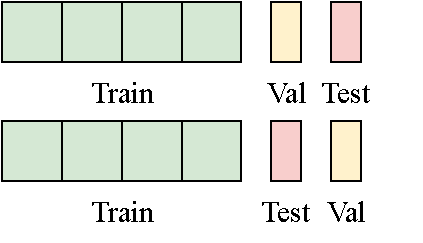
\includegraphics[scale=0.6]{figs/test_val_split.pdf}
  \caption[Splitting $kth$ fold]{Splitting $kth$ fold into a test and val set for hyperparameter optimisation \\ (run once on top configuration and once on bottom)}
\end{figure}

\subsubsection{Labelled splits}
While the datasets used in this project include labels for all the samples, the focus of this project is on semi-supervised learning.
In order to give an overall view of the performance for each dataset I performed evaluation of the models with different amounts of
labelled data. For each number of labelled samples ($n$) used, I selected $n$ samples from the train set in a stratified way to use as the 
labelled dataset. The unlabelled dataset was then all the remaining samples in the train set.

\subsubsection{Parallelisation}
While cross-validation reduces the number of iterations to a more manageable size, even a model with a fairly short 
training time will take a long time to complete the evaluation. Therefore I computed the indices of test/val/train and labelled 
splits I would use in advance, and serialised these using \texttt{pickle} \footnote{\texttt{pickle} is the most popular Python library 
for serialisation}. This allows all the models to use the same folds, allowing
for a fair comparison. It also allows each script to run hyperparameter optimisation over only one fold. The Cambridge High Performance
Cluster has 90 GPUs, and so running many smaller jobs in parallel gives a much quicker finish time than running several larger jobs.
I wrote several \texttt{bash} scripts to schedule slurm jobs for each model, number of labelled examples and fold. 

\section{Saliency} \label{saliency}
Neural networks are a black box, giving no indication to the programmer or user of what the network is doing, and what it deems 
to be important. One way of extracting that is through saliency maps (first introduced in~\cite{DBLP:journals/corr/SimonyanVZ13}), 
which intend to give the user some idea of which inputs 
are the most important in determining the output class. This is done by computing the partial derivatives of the input data 
with respect to the output class of the network. If the input values have been scaled to have similar ranges then this partial derivative
should be larger for inputs that are more important to determining the class. A large positive partial derivative means that increasing 
the value of that input makes the class more likely; and a large negative partial derivative means increasing that input decreases the 
likelihood of that class.

A variant of this uses guided backpropagation~\cite{DBLP:journals/corr/SpringenbergDBR14}, a variant of backpropagation where the 
gradient is only backpropagated through a ReLU if the error gradient is greater than zero. When used to construct saliency maps for 
images it has been shown to make much clearer images, and highlight better the features the network thinks are important.

I implemented both of these methods, basing my implementation on this very simple implementation: https://github.com/Ema93sh/pytorch-saliency.
The guided backpropagation version works by registering a hook on each ReLU module that sets the gradient being backpropagated 
to zero if it is less than zero.

\section{Command line tool}
One of the success criteria of this project was to build a tool, and so the \texttt{main.py} file in the repository provides a command line tool 
for building a semi-supervised learning model. The tool uses many of the techniques described earlier in this section, but many of the 
decisions made are based on results in the evaluation section, so the description of the tool is in Section~\ref{tool}.

\section{Repository overview}

\begin{figure}[H]
    \centering
    \begin{minipage}{7cm}
        \dirtree{%
        .1 +Semi-Supervised\_Models.
        .2 main.py.
        .2 requirements.txt.
        .2 +Models.
        .3 Model.py.
        .3 Simple.py.
        .3 M1.py.
        .3 SDAE.py.
        .3 M2.py.
        .3 Ladder.py.
        .3 +BuildingBlocks.
        .2 Saliency.
        .2 scripts.
        .2 utils.
        }
    \end{minipage}
    \caption{Directory structure of the repository}
\end{figure}

The top level of the repository contains the files \texttt{main.py} and \texttt{requirements.txt}. These are the script for running the tool,
and the packages I am using in the virtual environment respectively. \texttt{Models} contains the code for the models,
including the base modules in \texttt{BuildingBlocks} and the abstract class \texttt{Model.py}.
\texttt{scripts} contains all the python and bash scripts used in 
for evaluation, but this folder was created for tidiness and the scripts have to be moved up one level into 
\texttt{Semi-Supervised\_Models} to be run. \texttt{utils} contains functions for loading data, along with the code for early stopping and 
making the MNIST and TCGA folds. \texttt{Saliency} contains all the code for generating saliency maps.